\documentclass[../CSC_5RO17_TA_TP1.tex]{subfiles}

\begin{document}
\subsection{Question 3}
\subsubsection{Direct Linear Transformation}
\noindent L'\textbf{homographie} est réécrite de la façon suivante:
\begin{equation*}
    \underbrace{
        \begin{bmatrix}
            x_{2}\\y_{2}\\1
        \end{bmatrix}
    }_{\mathbf{x}_{\pi_{2}}}
    =
    \underbrace{
        \begin{bmatrix}
            h_{11} & h_{12} & h_{13}\\
            h_{21} & h_{22} & h_{23}\\
            h_{31} & h_{32} & h_{33}\\
        \end{bmatrix}
    }_{\mathbf{H}}
    \underbrace{
        \begin{bmatrix}
            x_{1}\\y_{1}\\1
        \end{bmatrix}
    }_{\mathbf{x}_{\pi_{1}}}
    \quad\to\quad
    \mathbf{x}_{\pi_{2}} =
    \begin{bmatrix}
        \mathbf{h}_{1}\\\mathbf{h}_{2}\\\mathbf{h}_{3}\\
    \end{bmatrix}
    \mathbf{x}_{\pi_{1}}
    \qquad\text{où}
    \begin{cases}
        \mathbf{h}_1 = \begin{bmatrix}h_{11} & h_{12} & h_{13}\end{bmatrix}\vspace{1mm}\\
        \mathbf{h}_2 = \begin{bmatrix}h_{21} & h_{22} & h_{12}\end{bmatrix}\vspace{1mm}\\
        \mathbf{h}_3 = \begin{bmatrix}h_{31} & h_{32} & h_{13}\end{bmatrix}\\
    \end{cases}
\end{equation*}
Ce qui peut être réécrit comme suit:
\begin{equation*}
    \left\{
    \begin{aligned}
        -\mathbf{h}_{1}\mathbf{x}_{\pi_{1}} &  & +x_{2}\mathbf{h}_{3}\mathbf{x}_{\pi_{1}} &= 0\\
         & -\mathbf{h}_{2}\mathbf{x}_{\pi_{1}} & +y_{2}\mathbf{h}_{3}\mathbf{x}_{\pi_{1}} &= 0\\
    \end{aligned}
    \right.
    \quad\xrightarrow{\mathbf{h} =\begin{bmatrix}\mathbf{h}_{1} & \mathbf{h}_{2} & \mathbf{h}_{3}\end{bmatrix}^\intercal}
    \left\{
    \begin{aligned}
        \underbrace{
            \begin{bmatrix}
                -\mathbf{x}_{\pi_{1}}^{\intercal} & +\mathbf{0}_{3}^{\intercal} & -x_{2}\mathbf{x}_{\pi_{1}}^{\intercal}
            \end{bmatrix}
        }_{\mathbf{a}_{x}}
        \mathbf{h} &= 0\\
        \underbrace{
            \begin{bmatrix}
                +\mathbf{0}_{3}^{\intercal} & -\mathbf{x}_{\pi_{1}}^{\intercal} & -y_{2}\mathbf{x}_{\pi_{1}}^{\intercal}
            \end{bmatrix}
        }_{\mathbf{a}_{y}}
        \mathbf{h} &= 0
    \end{aligned}
    \right.
\end{equation*}
Ce système est valable pour toutes les paires de points $N$, de sorte que l'équation peut être écrite comme suit:
\begin{equation}
    \underbrace{
        \begin{bmatrix}
            -x_{1_{\pi_1}} & -y_{1_{\pi_1}} & -1 & 0 & 0 & 0 & x_{1_{\pi_2}}x_{1_{\pi_1}} & x_{1_{\pi_2}}y_{1_{\pi_1}} & x_{1_{\pi_2}}\\
            0 & 0 & 0 & -x_{1_{\pi_1}} & -y_{1_{\pi_1}} & -1 & y_{1_{\pi_2}}x_{1_{\pi_1}} & y_{1_{\pi_2}}y_{1_{\pi_1}} & y_{1_{\pi_2}}\\
            \vdots&\vdots&\vdots&\vdots&\vdots&\vdots&\vdots&\vdots&\vdots\\
            -x_{i_{\pi_1}} & -y_{i_{\pi_1}} & -1 & 0 & 0 & 0 & x_{i_{\pi_2}}x_{i_{\pi_1}} & x_{i_{\pi_2}}y_{i_{\pi_1}} & x_{i_{\pi_2}}\\
            0 & 0 & 0 & -x_{i_{\pi_1}} & -y_{i_{\pi_1}} & -1 & y_{i_{\pi_2}}x_{i_{\pi_1}} & y_{i_{\pi_2}}y_{i_{\pi_1}} & y_{i_{\pi_2}}\\
            \vdots&\vdots&\vdots&\vdots&\vdots&\vdots&\vdots&\vdots&\vdots\\
            -x_{N_{\pi_1}} & -y_{N_{\pi_1}} & -1 & 0 & 0 & 0 & x_{N_{\pi_2}}x_{N_{\pi_1}} & x_{N_{\pi_2}}y_{N_{\pi_1}} & x_{N_{\pi_2}}\\
            0 & 0 & 0 & -x_{N_{\pi_1}} & -y_{N_{\pi_1}} & -1 & y_{N_{\pi_2}}x_{N_{\pi_1}} & y_{N_{\pi_2}}y_{N_{\pi_1}} & y_{N_{\pi_2}}\\
        \end{bmatrix}
    }_{\mathbf{A}\;(2N\times9)}
    \underbrace{
        \begin{bmatrix}
            h_{11}\\h_{12}\\h_{13}\\h_{21}\\h_{22}\\h_{23}\\h_{31}\\h_{32}\\h_{33}
        \end{bmatrix}
    }_{\mathbf{h}\;(9\times1)}
    =
    \begin{bmatrix}
        0\\0\\0\\0\\0\\0\\0\\0\\0\\
    \end{bmatrix}
\end{equation}
Ce qui peut être résolu à l'aide de la méthode des SVD.
\begin{scriptsize}\mycode
    \lstinputlisting[
        caption=Extrait de code du fichier \texttt{q3.py},
        language=Python,
        firstline=39,
        lastline=41,
    ]{../../src/q3.py}
\end{scriptsize}

\subsubsection{Normalisation}
\noindent Par contre, cette méthode présentera des erreurs de plus en plus importantes à mesure que la taille de l'image augmente. Ainsi, la normalisation des coordonnées peut être appliquée pour éliminer la dépendance entre l'estimation de l'homographie et la taille de l'image à l'aide de l'opérateur suivant:
\begin{equation}
    \boxed{
        \mathbf{T}
        =
        \begin{bmatrix}
            \frac{2}{w} & 0 & -1\\
            0 & \frac{2}{h} & -1\\
            0 & 0 & +1\\
        \end{bmatrix}
    }
\end{equation}
Où $w$ est la largeur de l'image et $h$ est la hauteur de l'image. Cet opérateur est simplement une combinaison de translation et de recadrage de l'image. La normalisation est appliquée de la manière suivante:
\begin{equation*}
    \left\{
    \begin{aligned}
        \widetilde{\mathbf{x}}_{i_{\pi_{1}}} &= \mathbf{T}\mathbf{x}_{i_{\pi_{1}}}\\
        \widetilde{\mathbf{x}}_{i_{\pi_{2}}} &= \mathbf{T}\mathbf{x}_{i_{\pi_{2}}}\\
        \mathbf{H} &= \mathbf{T}^{-1}\widetilde{\mathbf{H}}\mathbf{T}\\
    \end{aligned}
    \right.
\end{equation*}
Après l'application de la normalisation sur les coordonnées des vecteurs, la méthode DLT est appliquée et son résultat doit être dénormalisé pour que l'homographie soit compatible avec le système de dimensions originales.

\subsubsection{L'Erreur de Reprojection}
\noindent L'erreur de reprojection est un indice de confiance utilisé pour évaluer la qualité et la fiabilité de l'homographie. Elle est définie par l'équation suivante:

\begin{equation}
    \boxed{
        E = \frac{1}{n} \sum_{i=1}^{n}\mathbf{e}_{i}
        \quad\text{où}\quad
        \mathbf{e}_{i} = \left\lVert \mathbf{p}_{p_{i}} - \mathbf{p}_{c_{i}} \right\rVert
    }
\end{equation}
Où $\mathbf{p}_{p_{i}}$ est un point $i$ projeté par l'homographie $\mathbf{H}$ et $\mathbf{p}_{c_{i}}$ est un point $i$ cible calculé précédemment.
\begin{remark}
    Les points originaux peuvent être reprojetés en utilisant cette matrice et comparés aux points correspondants réels. Plus l'erreur de reprojection est petite, plus l'homographie est fiable.
\end{remark}

\noindent Après l'implémentation en Python des algorithmes présentés précédemment, les résultats suivants sont obtenus:
\begin{figure}[H]
    \centering
    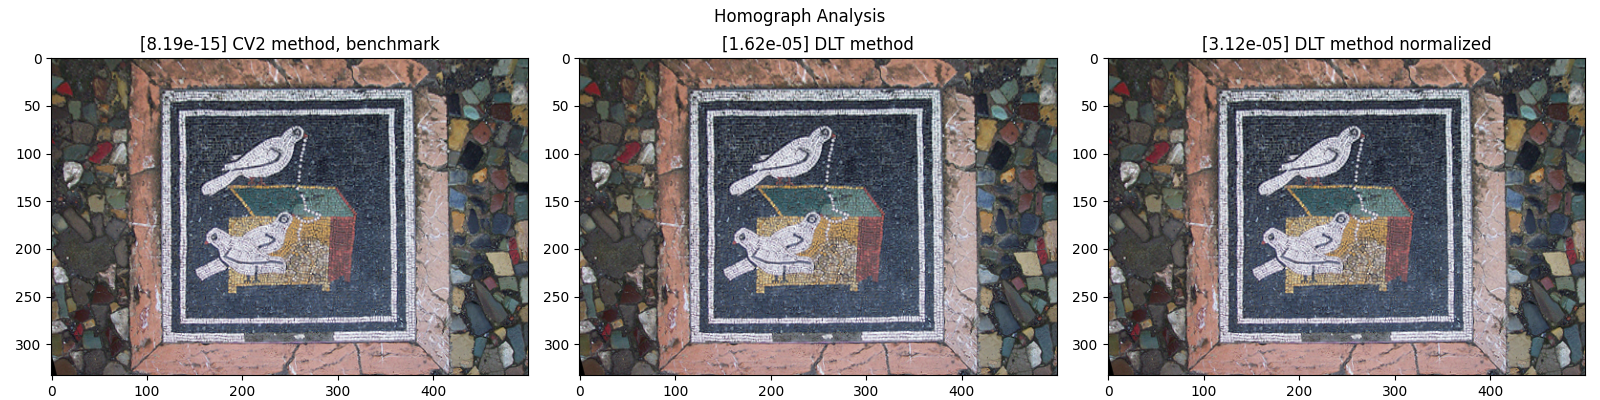
\includegraphics[width=\linewidth]{../../data/output/CSC_5RO17_TP1_Q3.png}
    \caption{Application Homographie}
    \label{fig_homography}
\end{figure}
Chaque image correspond à une méthode appliquée pour obtenir l'homographie désirée. Entre crochet, l'erreur de reprojection de chaque méthode est indiquée.
\begin{remark}
    Le résultat obtenu avec OpenCV est ajouté à l'image ci-dessus comme référence d'un résultat idéal.
    \begin{scriptsize}\mycode
        \lstinputlisting[caption=Extrait de code du fichier \texttt{q3.py},language=Python, firstline=47, lastline=49]{../../src/q3.py}
    \end{scriptsize}
\end{remark}
\noindent Il est notable que la méthode utilisée avec OpenCV est beaucoup plus efficace, car son erreur de reprojection est la plus faible parmi les méthodes testées.\\

\noindent Il est également remarquable que la normalisation n'a pas réduit l'erreur ; au contraire, elle l'a doublée. Il est possible que, étant donné la taille relativement petite de l'image, l'influence de la taille sur l'erreur de calcul soit moins significative que l'erreur causée par l'inversion de la matrice $\textbf{T}$ nécessaire pour la dénormalisation.
\end{document}
